\documentclass[tikz,margin=2mm]{standalone}
\pagestyle{empty}

%\usepackage{aistats2020}
\usepackage{amsmath}
\usepackage{bm}
\usetikzlibrary{positioning,calc, arrows}

% variable styles
\tikzstyle{error} = [ draw=black,fill=gray!50!white,circle, inner sep = 1pt, minimum size = 0.35cm ]
\tikzstyle{latent} = [ draw, circle, inner sep = 2pt, minimum size = 0.65cm ]
\tikzstyle{observed} = [ draw, rectangle, inner sep = 2pt, minimum size = 0.65cm ]
\tikzstyle{measure} = [ draw, rectangle, inner sep = 0pt, minimum size = 0.45cm, outer sep = 0.5pt]
\tikzstyle{refpoint} = [inner sep = 0pt, outer sep = 0pt]


\tikzstyle{edge} = [->]
\tikzstyle{highlightEdge} = [->, very thick]
\tikzstyle{highlightEdge2} = [->, dashed]
\tikzstyle{transform} = [->, very thick, >=triangle 45]


\begin{document}

%%%%%%%%%%%%%%%% Original Figure 1 %%%%%%%%%%%%%%%%%%%%%%%%%%%%%%%%%%%

% F=Adapted from book Principles and Practice of SEM by Kline, p. 280.
% SEM from Shen, B.-J., & Takeuchi, D.T. (2001). A structural model of acculturation and
% mental health status among Chinese Americans. American Journal of Community Psychology,
% 29, 387-418.

% \begin{tikzpicture}[scale=0.9]
% 	
% 	\begin{scope}
% 	
% 		\fill[ fill=gray!30!white, anchor = north west ] (-0.15,1.5) rectangle +(3.3,-2.35);
% 	
% 		\node[anchor=north west] at (-0.15,1.5) {\itshape \small latent level};
% 		\node[anchor=north east] at (-0.15,1.5) {\itshape \small observed level};
% 	
% 	
% 		\node[latent, text width=1cm, align = center, fill=white] (ses) at (0.7,0) {SES};
% 		\node[latent, text width=1cm, align = center, fill=white] (stress) at (2.3,0) {Stress};
% 		\node[observed, text width = 2cm, align=center] (depression) at (1.5,-1.5){Depression Scale};
% 		\draw[edge, <->] (ses) -- (stress);
% 		\draw[edge] (ses) -- (depression);
% 		\draw[edge] (stress) -- (depression);
% 		
% 		% Measurements of ses
% 		\begin{scope}[xshift=-1.5cm, yshift=0cm]
% 			\node[observed,  text width=2cm, align=center] (edu) at (0,-0.5) {Education};
% 			\node[observed, text width=2cm, align=center] (inc) at (0,0.5) {Income};
% 			\draw[edge] (ses) -- (edu.east);
% 			\draw[edge] (ses) -- (inc.east);
% 		\end{scope}
% 		
% 		% Measurements of stress
% 		\begin{scope}[xshift=4.5cm, yshift=0cm]
% 			\node[observed, text width=2cm, align=center] (ip) at (0,-0.5) {Interpersonal};
% 			\node[observed, text width=2cm, align=center] (job) at (0,0.5) {Job};
% 			\draw[edge] (stress) -- (ip.west);
% 			\draw[edge] (stress) -- (job.west);
% 		\end{scope}
% 		
% 		
% 		%\node at (0,-1.8) {(a)};
% 	
% 	\end{scope}
% 
% \end{tikzpicture}

% Page 1: Democracy example from Bollen 1996
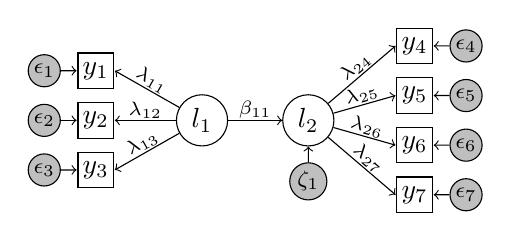
\begin{tikzpicture}[scale=0.9]
	\node[latent] (xi1) at (1.5, 0) {$ \l_1 $};
	\node[latent] (eta1) at (3, 0) {$ \l_2 $};
	\node[measure] (x1) at ( 0, 0.7) {$ y_1 $};
	\node[measure] (x2) at ( 0, 0) {$ y_2 $};
	\node[measure] (x3) at ( 0, -0.7) {$ y_3 $};
	\node[measure] (y1) at ( 4.5, 1.05) {$ y_4 $};
	\node[measure] (y2) at ( 4.5, 0.35) {$ y_5 $};
	\node[measure] (y3) at ( 4.5, -0.35) {$ y_6 $};
	\node[measure] (y4) at ( 4.5, -1.05) {$ y_7 $};

	\node[error] (zeta1) [below=.2cm of eta1] {\footnotesize $ \zeta_1 $};
	\node[error] (e1) [right=.2cm of y1] {\footnotesize $ \epsilon_4 $};
	\node[error] (e2) [right=.2cm of y2] {\footnotesize $ \epsilon_5 $};
	\node[error] (e3) [right=.2cm of y3] {\footnotesize $ \epsilon_6 $};
	\node[error] (e4) [right=.2cm of y4] {\footnotesize $ \epsilon_7 $};
	\node[error] (d1) [left=.2cm of x1] {\footnotesize $ \epsilon_1 $};
	\node[error] (d2) [left=.2cm of x2] {\footnotesize $ \epsilon_2 $};
	\node[error] (d3) [left=.2cm of x3] {\footnotesize $ \epsilon_3 $};

	\draw[edge](xi1) -- (eta1) node[midway, above, sloped, yshift=-0.1cm]{\scriptsize $ \beta_{11} $};
	\draw[edge](xi1) -- (x1.east) node[midway, above, sloped, yshift=-0.1cm]{\scriptsize $ \lambda_{11} $};
	\draw[edge](xi1) -- (x2.east) node[midway, above, sloped, yshift=-0.1cm]{\scriptsize $ \lambda_{12} $};
	\draw[edge](xi1) -- (x3.east) node[midway, above, sloped, yshift=-0.1cm]{\scriptsize $ \lambda_{13} $};
	\draw[edge](eta1) -- (y1.west) node[midway, above, sloped, yshift=-0.1cm]{\scriptsize $ \lambda_{24} $};
	\draw[edge](eta1) -- (y2.west) node[midway, above, sloped, yshift=-0.1cm]{\scriptsize $ \lambda_{25} $};
	\draw[edge](eta1) -- (y3.west) node[midway, above, sloped, yshift=-0.1cm]{\scriptsize $ \lambda_{26} $};
	\draw[edge](eta1) -- (y4.west) node[midway, above, sloped, yshift=-0.1cm]{\scriptsize $ \lambda_{27} $};
	\draw[edge](e1) -- (y1);
	\draw[edge](e2) -- (y2);
	\draw[edge](e3) -- (y3);
	\draw[edge](e4) -- (y4);
	\draw[edge](d1) -- (x1);
	\draw[edge](d2) -- (x2);
	\draw[edge](d3) -- (x3);
	\draw[edge](zeta1) -- (eta1);

\end{tikzpicture}

% Page 2
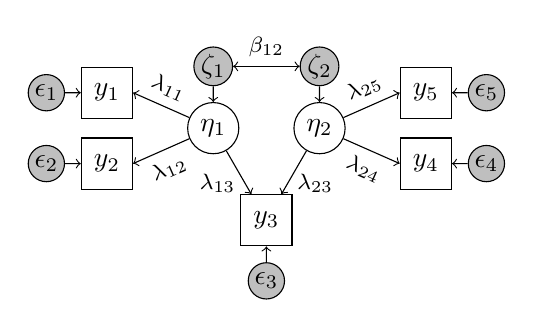
\begin{tikzpicture}[scale=0.9]
	
	\begin{scope}
	
		%\fill[ fill=gray!30!white, anchor = north west ] (-0.3,1.5) rectangle +(3.6,-2.35);
	
		%\node[anchor=north west] at (-0.3,1.5) {\itshape \small latent level};
		%\node[anchor=north east] at (-0.3,1.5) {\itshape \small observed level};

		\node[latent] (ses) at (0.5,0) {$\eta_1$};
		\node[latent] (stress) at (2,0) {$\eta_2$};
		\node[observed] (depression) at (1.25,-1.3){$y_3$};
		
		
		% \draw[edge, <->] (ses) -- (stress) node[midway,above ] {\footnotesize $\beta_{12}$};
		\draw[edge] (ses) -- (depression) node[near end,left] {\footnotesize $\lambda_{13}$};
		\draw[edge] (stress) -- (depression) node[near end, right] {\footnotesize $\lambda_{23}$};
		
		% errors
		\node[error, inner sep=.5pt ] (zeta1) [above=.2cm of ses]  {$ \zeta_1 $};
		\node[error, inner sep=.5pt ] (zeta2) [above=.2cm of stress]  {$ \zeta_2 $};
		\node[error] (err3) [below=.2cm of depression]{$ \epsilon_3 $};
		\draw[edge] (err3) -- (depression);
		\draw[edge] (zeta1) -- (ses);
		\draw[edge] (zeta2) -- (stress);
		\draw[edge, <->] (zeta1) -- (zeta2) node[midway,above] {\footnotesize $ \beta_{12} $};	
		
		% Measurements of ses
		\begin{scope}[xshift=-1cm, yshift=0cm]
		
			\node[observed] (edu) at (0,-0.5) {$y_2$};
			\node[observed] (inc) at (0,0.5) {$y_1$};
			\draw[edge] (ses) -- (edu.east) node[midway, below, sloped ] {\footnotesize $\lambda_{12}$ };
			\draw[edge] (ses) -- (inc.east) node[midway, above, sloped ] {\footnotesize $\lambda_{11}$ };
			
			%errors
			\node[error] (err2) [left=.2cm of edu] {$ \epsilon_2 $};
			\node[error] (err1) [left=.2cm of inc] {$ \epsilon_1 $};
			\draw[edge] (err2) -- (edu);
			\draw[edge] (err1) -- (inc);
			
			%crossloading on income and education
			% \draw[edge, <->] (err2) -- (err1);
			
		\end{scope}
		
		% Measurements of stress
		\begin{scope}[xshift=3.5cm, yshift=0cm]
			\node[observed] (ip) at (0,-0.5) {$y_4$};
			\node[observed] (job) at (0,0.5) {$y_5$};
			\draw[edge] (stress) -- (ip.west) node[midway, below, sloped ] {\footnotesize $\lambda_{24}$ };
			\draw[edge] (stress) -- (job.west) node[midway, above, sloped ] {\footnotesize $\lambda_{25}$ };
			
			%errors
			\node[error] (err4) [right=.2cm of ip] {$ \epsilon_4 $};
			\node[error] (err5) [right=.2cm of job] {$ \epsilon_5 $};
			\draw[edge] (err4) -- (ip);
			\draw[edge] (err5) -- (job);
		\end{scope}
		
		
		%\node at (0,-1.8) {(a)};
	
	\end{scope}

\end{tikzpicture}
% % Page 2
% \begin{tikzpicture}[scale=0.9]
% 	\begin{scope}	
% 		\node[latent] (ses) at (0,-0.5) {$l_1$};
% 		\node[latent] (stress) at (0,0.5) {$l_2$};
% 		\node[measure] (depression) at (1.2,0){$y_3$};
% 			
% 		%\draw[edge, <->] (ses) -- (stress) node[midway,above ] {\footnotesize $\beta_{12}$};
% 		\draw[edge] (ses) -- (depression);
% 		\draw[edge] (stress) -- (depression);
% 		
% 		% errors
% 		\node[error, inner sep=.5pt ] (zeta1) [left=.1cm of ses]  {\footnotesize $ \zeta_1 $};
% 		\node[error, inner sep=.5pt ] (zeta2) [left=.1cm of stress]  {\footnotesize $ \zeta_2 $};
% 		\node[error] (err3) [below=.1cm of depression]{\footnotesize $ \epsilon_3 $};
% 		\draw[edge] (err3) -- (depression);
% 		\draw[edge] (zeta1) -- (ses);
% 		\draw[edge] (zeta2) -- (stress);
% 		\draw[edge, <->] (zeta1) -- (zeta2);	
% 			
% 		% Measurements of ses
% 		\begin{scope}[xshift=0cm, yshift=-1.5cm]	
% 			\node[measure] (edu) at (0.5,0) {$y_2$};
% 			\node[measure] (inc) at (-0.5,0) {$y_1$};
% 			\draw[edge] (ses) -- (edu);
% 			\draw[edge] (ses) -- (inc);
% 			
% 			%errors
% 			\node[error] (err2) [below=.1cm of edu] {\footnotesize $ \epsilon_2 $};
% 			\node[error] (err1) [below=.1cm of inc] {\footnotesize $ \epsilon_1 $};
% 			\draw[edge] (err2) -- (edu);
% 			\draw[edge] (err1) -- (inc);
% 			
% 			%crossloading on income and education
% 			% \draw[edge, <->] (err2) -- (err1);	
% 		\end{scope}
% 		
% 		% Measurements of stress
% 		\begin{scope}[xshift=0cm, yshift=1.5cm]
% 			\node[measure] (ip) at (0.5,0) {$y_4$};
% 			\node[measure] (job) at (-0.5,0) {$y_5$};
% 			\draw[edge] (stress) -- (ip);
% 			\draw[edge] (stress) -- (job);
% 			
% 			%errors
% 			\node[error] (err4) [above=.1cm of ip] {\footnotesize $ \epsilon_4 $};
% 			\node[error] (err5) [above=.1cm of job] {\footnotesize $ \epsilon_5 $};
% 			\draw[edge] (err4) -- (ip);
% 			\draw[edge] (err5) -- (job);
% 		\end{scope}	
% 	\end{scope}
% 	
% \end{tikzpicture}

% Page 3: The equations belonging to the SEM of the previous figure.
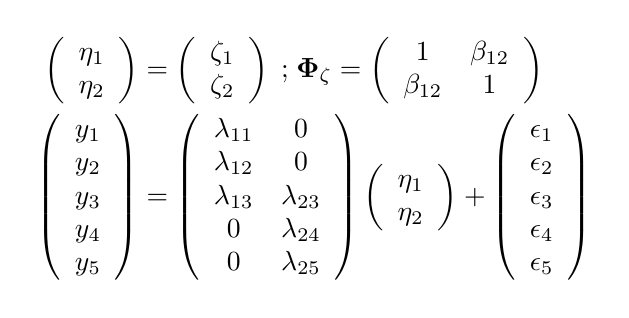
\begin{tikzpicture}[scale=0.9]

	\node (eq1) at (0,0) {

		$ 
		\begin{aligned}
		\left( \begin{array}{c}
			\eta_1 \\
			\eta_2 \end{array} \right) &= 
		\left( \begin{array}{c}
			\zeta_1 \\
			\zeta_2 \end{array} \right) \; \mathbf{;} \;
		\bm{\Phi}_\zeta = 
			\left( \begin{array}{cc}
				1 & \beta_{12} \\
				\beta_{12} & 1 \end{array} \right) \\
		\left( \begin{array}{c}
			y_1 \\
			y_2 \\
			y_3 \\
			y_4 \\
			y_5 \end{array} \right) &= 
		\left( \begin{array}{cc}
			\lambda_{11} & 0 \\
			\lambda_{12} & 0 \\
			\lambda_{13} & \lambda_{23} \\
			0 & \lambda_{24} \\
			0 & \lambda_{25} \end{array} \right) 
		\left( \begin{array}{c}
			\eta_1 \\
			\eta_2 \end{array} \right) +
		\left( \begin{array}{c}
			\epsilon_1 \\
			\epsilon_2 \\
			\epsilon_3 \\
			\epsilon_4 \\
			\epsilon_5 \end{array} \right) \\
		\end{aligned}
		$
	};
	
	
\end{tikzpicture}

% Page 4
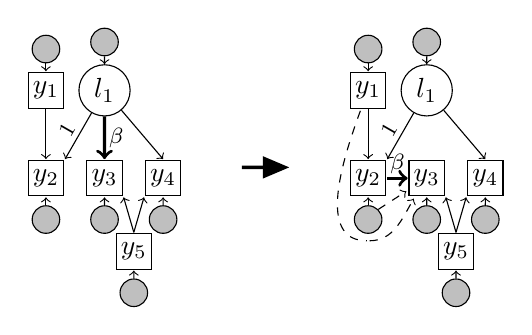
\begin{tikzpicture}[scale=0.93]
	\begin{scope}	
	    \node [latent]  (xi2)   at (0.8,0) {$l_1$};
	    %\node [latent] (zeta_xi) [above=0.25cm of xi] {$ \epsilon_\xi $};
	    \node [measure] (xi1) at (0,0) {$y_1$};
	    \node [error] (ey1) [above = .1cm of xi1] {};
	    \node [error] (ex1) [above = .1cm of xi2] {};
	    \draw[edge] (ey1) -- (xi1);
	    \draw[edge] (ex1) -- (xi2);
	    
	    \begin{scope}[yshift = -1.2cm ]
			\node [measure] (x1) at (0,0) {$y_2$};
			\node [measure] (x2) at (0.8,0){$y_3$};
			\node [measure] (x3) at (1.6,0){$y_4$};
			% \node [measure] (x4) at (3,0){$x_6$};
	    \end{scope}
	    
	    \draw[edge] (xi2) -- (x1.north east) node[sloped, midway, above, yshift=-0.05cm] { \footnotesize $ 1 $ };
	    \draw[highlightEdge] (xi2)      -- (x2.north) node[midway,right, xshift=-0.08cm] { \footnotesize $ \mathbf{\beta} $ };
	    \draw[edge] (xi2)      -- (x3.north);
	    % \draw[edge] (xi2)      -- (x4.north west);
	    \draw[edge] (xi1) -- (x1.north);
	    
	    \begin{scope}[yshift = -1.8cm ]
		    	\node [error] (e1) [below=.1cm of x1] {};
			\node [error] (e2) [below=.1cm of x2] {};
			\node [error] (e3) [below=.1cm of x3] {};
			% \node [error] (e4) at (3,0){};
			\node [measure] (xi3) at (1.2,-0.4){$y_5$};
			\node [error] (e6) [below =.1cm of xi3 ]{};
	    \end{scope}
	    
	    \draw[edge] (e1) -- (x1.south);
	    \draw[edge] (e2) -- (x2.south);
	    \draw[edge] (e3) -- (x3.south);
	    % \draw[edge] (e4) -- (x4.south);
	    \draw[edge] (e6) -- (xi3);
	    \draw[edge] (xi3.north) -- (x2.south east);
	    \draw[edge] (xi3.north) -- (x3.south west);
	
	
	\end{scope}
	
	\begin{scope}[xshift = 4.4cm]
	
		\node [latent]  (xi2)   at (0.8,0) {$l_1$};
	    %\node [latent] (zeta_xi) [above=0.25cm of xi] {$ \epsilon_\xi $};
	    \node [measure] (xi1) at (0,0) {$y_1$};
	    \node [error] (ey1) [above = .1cm of xi1] {};
	    \node [error] (ex1) [above = .1cm of xi2] {};
	    \draw[edge] (ey1) -- (xi1);
	    \draw[edge] (ex1) -- (xi2);
	    
	    \begin{scope}[yshift = -1.2cm ]
			\node [measure] (x1) at (0,0) {$y_2$};
			\node [measure] (x2) at (0.8,0){$y_3$};
			\node [measure] (x3) at (1.6,0){$y_4$};
			% \node [measure] (x4) at (3,0){$x_6$};
			\draw [highlightEdge] (x1) to (x2); 
			\node [refpoint] (betax) at ($(x1)!0.5!(x2)$){};
			\node [above=1pt of betax, outer sep = 0pt, inner sep = 0pt] { \footnotesize $\mathbf{\beta}$};
			%\node[midway] { };
	    \end{scope}
	    
		\draw[edge] (xi2) -- (x1.north east) node[sloped, midway, above, yshift=-0.05cm] { \footnotesize $ 1 $ };
	    \draw[edge] (xi2)      -- (x3.north);
	    % \draw[edge] (xi2)      -- (x4.north west);
	    \draw[edge] (xi1) -- (x1.north);
	    
	    
		\begin{scope}[yshift = -1.8cm ]
			\node [error] (e1) [below=.1cm of x1] {};
			\node [error] (e2) [below=.1cm of x2] {};
			\node [error] (e3) [below=.1cm of x3] {};
			% \node [error] (e4) at (3,0){};
			\node [measure] (xi3) at (1.2,-0.4){$y_5$};
			\node [error] (e6) [below =.1cm of xi3 ]{};
	    \end{scope}
	    
	    \draw[edge] (e1) -- (x1.south);
	    \draw[edge] (e2) -- (x2.south);
	    \draw[edge] (e3) -- (x3.south);
	    % \draw[edge] (e4) -- (x4.south);
	    \draw[edge] (e6) -- (xi3);
	    \draw[edge] (xi3.north) -- (x2.south east);
	    \draw[edge] (xi3.north) -- (x3.south west);
	    
	    \node[refpoint] (start1) [left = 0.75mm of xi1.south ] {};
	    \node[refpoint] (mid1) [below = 2pt of e1.south] {};
	    \node[refpoint] (end2) [above = 2pt of x2.south west] {};
	    \node[refpoint] (end1) [right = 2pt of x2.south west] {};
		
	    \draw [highlightEdge2] (start1) to [out=-110,in=180] (mid1) to [out=0,in=-120] (end1);
	    \draw [highlightEdge2] (e1.north east) to (end2);
	
	
	\end{scope}
	
	%\node at (4.25,-3.2) {(a)};
	%\draw [transform] (3.4,-1.25) -- (4,-1.25);
	\node (arrowStart) [left=.3cm of current bounding box.center] {};
	\node (arrowEnd) [right=.3cm of current bounding box.center] {};
	
	\draw [transform] (arrowStart) -- (arrowEnd);
	
	
\end{tikzpicture}

% Page 5
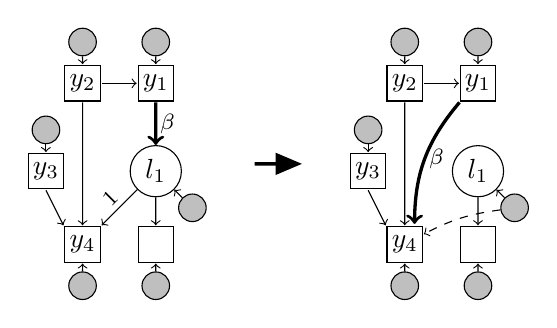
\begin{tikzpicture}[scale=0.93]

	%\clip (-0.5,0.5) rectangle +(8.5,-4);

	\begin{scope}
	
	  %Node
	    \node [measure] (y2)   at (1.5,0) {$y_1$};
	    \node [measure] (y1) at (0.5,0)  {$y_2$};
	    %\node [error] (e1) at (2.3,0) {};
	    \node [error] (ey1) [above = .1cm of y1] {};
	    \draw[edge] (ey1) -- (y1);
	    \node [error] (ey2) [above = .1cm of y2] {};
	    \draw[edge] (ey2) -- (y2);
	
	
		\begin{scope}[yshift =-1.2cm]
			\node[latent] (x1) at (1.5,0){$l_1$};
			\node[error] (z2) at (2,-0.5){};
			\node[measure] (y3) at (0,0){$y_3$};
			\node[error] (ey3) [above=.1cm of y3] {};
			\draw[edge] (ey3) -- (y3);
		\end{scope}
		
		\begin{scope}[yshift =-2.2cm]
			\node[measure] (y4) at (0.5,0){$y_4$};
			\node[measure] (y5) at (1.5,0){};
			% \node[measure] (y6) at (2.5,0){};
			
			\node[error] (e3) [below=.1cm of y4] {};
			\node[error] (e4) [below=.1cm of y5] {};
			% \node[error] (e5) at (2.5,-0.7){};
		\end{scope}
	
	
		\draw[edge] (y1) -- (y2);
		\draw[edge] (y1) -- (y4);
		\draw[edge] (y3.south) -- (y4.north west);
		\draw[highlightEdge] (y2) -- (x1) node [midway,right,xshift=-0.08cm]{\footnotesize $\mathbf{\beta}$};
		
		\draw[edge] (x1) -- (y4) node[sloped, midway, above, yshift=-0.05cm] { \footnotesize $ 1 $ };
		\draw[edge] (x1) -- (y5);
		% \draw[edge] (x1) -- (y6);
	
		%\draw[edge] (e1) -- (y2.east);
		\draw[edge] (z2) -- (x1);
		\draw[edge] (e3) -- (y4);
		\draw[edge] (e4) -- (y5);
		% \draw[edge] (e5) -- (y6);
	
	
	\end{scope}
	
	%\node at (4.25,-8) {(b)};
	%\draw [transform] (3.3,-1.5) -- (4,-1.5);
	
	\begin{scope} [xshift=4.4cm]
	
	  %Node
	    \node [measure] (y2)   at (1.5,0) {$y_1$};
	    \node [measure] (y1) at (0.5,0)  {$y_2$};
	    %\node [error] (e1) at (2.3,0) {};
	    \node [error] (ey1) [above = .1cm of y1] {};
	    \draw[edge] (ey1) -- (y1);
	    \node [error] (ey2) [above = .1cm of y2] {};
	    \draw[edge] (ey2) -- (y2);
	
	
		\begin{scope}[yshift =-1.2cm]
			\node[latent] (x1) at (1.5,0){$l_1$};
			\node[error] (e2) at (2,-0.5){};
			\node[measure] (y3) at (0,0){$y_3$};
			\node[error] (ey3) [above=.1cm of y3] {};
			\draw[edge] (ey3) -- (y3);
		\end{scope}
		
		\begin{scope}[yshift =-2.2cm]
			\node[measure] (y4) at (0.5,0){$y_4$};
			\node[measure] (y5) at (1.5,0){};
			% \node[measure] (y6) at (2.5,0){};
			
			\node[error] (e3)[below=.1cm of y4] {};
			\node[error] (e4)[below=.1cm of y5] {};
			% \node[error] (e5) at (2.5,-0.7){};
		\end{scope}
	
	
		\draw[edge] (y1) -- (y2);
		\draw[edge] (y1) -- (y4);
		\draw[edge] (y3.south) -- (y4.north west);
		% \draw[edge] (y2) -- (x1); 
		\node[refpoint, right = 3pt of y4.north] (end1){};
		
		\draw [highlightEdge] (y2) edge [bend right=20] node [midway,right,inner
		sep = 1pt] {\footnotesize $\mathbf{\beta}$} (end1);
		\draw [highlightEdge2] (e2) edge [bend right = 10] (y4);
		
		
		% \draw[edge] (x1) -- (x1) node[midway, sloped, above] { 1 };
		\draw[edge] (x1) -- (y5);
		% \draw[edge] (x1) -- (y6);
	
		%\draw[edge] (e1) -- (y2.east);
		\draw[edge] (e2) -- (x1);
		\draw[edge] (e3) -- (y4);
		\draw[edge] (e4) -- (y5);
		% \draw[edge] (e5) -- (y6);
	
	
	\end{scope}
	
	
	\node (arrowStart) [left=.3cm of current bounding box.center] {};
	\node (arrowEnd) [right=.3cm of current bounding box.center] {};
	
	\draw [transform] (arrowStart) -- (arrowEnd);
	
\end{tikzpicture}

% Page 6
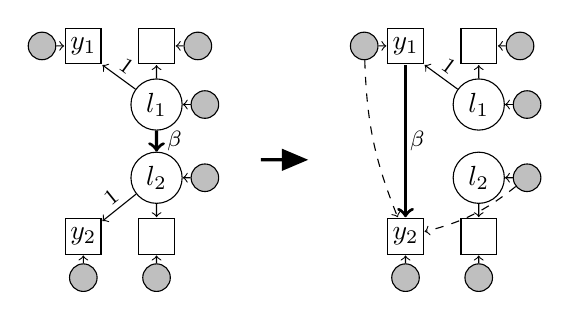
\begin{tikzpicture}[scale=0.93]
	
	\begin{scope}
	
		\node[measure] (y1) at (0.5,-0.6){$y_1$};
		\node[measure] (y2) at (1.5,-0.6){};
		% \node[measure] (y3) at (2.5,-0.6){};
		\node[error] (e1) [left=0.1cm of y1] {};
		\node[error] (e2) [right=0.1cm of y2] {};
		% \node[error] (e3) at (2.5,0){};
		
		\begin{scope}[yshift=-1.4cm]
			\node[latent] (xi1) at (1.5,0) {$l_1$};
			\node[error] (exi1) [right=.1cm of xi1] {};
			\draw[edge] (exi1) -- (xi1);
			\node[latent] (eta1) at (1.5,-1) {$l_2$};
			\node[error] (eeta) [right=.1cm of eta1] {};
		\end{scope}
		
		\begin{scope}[yshift=-3.2cm]
			\node[measure] (y4) at (0.5,0){$y_2$};
			\node[measure] (y5) at (1.5,0){};
			% \node[measure] (y6) at (2.5,0){};
			
			\node[error] (e4) [below=0.1cm of y4]{};
			\node[error] (e5) [below=0.1cm of y5]{};
			% \node[error] (e6) at (2.5,-0.6){};
		\end{scope}
		
		\draw[edge] (e1) -- (y1);
		\draw[edge] (e2) -- (y2);
		% \draw[edge] (e3) -- (y3);
		\draw[edge] (e4) -- (y4);
		\draw[edge] (e5) -- (y5);
		% \draw[edge] (e6) -- (y6);
		\draw[edge] (eeta) -- (eta1);
		
		\draw[edge] (xi1) -- node [midway, above, sloped, yshift=-0.05cm] {\footnotesize 1} (y1.south east);
		\draw[edge] (xi1) -- (y2);
		% \draw[edge] (xi1) -- (y3);
		
		\draw[edge] (eta1) -- node [midway, above, sloped, yshift=-0.05cm] {\footnotesize 1} (y4);
		\draw[edge] (eta1) -- (y5);
		% \draw[edge] (eta1) -- (y6);
		
		\draw[highlightEdge] (xi1) -- node [midway,right]{\footnotesize \textbf{$\beta$}} (eta1);
	
	\end{scope}
	
	%\draw [transform] (3.75,-11.5) -- (4.75,-11.5);
	
	\begin{scope}[xshift=4.4cm]
	
		\node[measure] (x1) at (0.5,-0.6){$y_1$};
		\node[measure] (x2) at (1.5,-0.6){};
		% \node[measure] (x3) at (2.5,-0.6){};
		\node[error] (e1) [left=0.1cm of x1] {};
		\node[error] (e2) [right=0.1cm of x2] {};
		
		\begin{scope}[yshift=-1.4cm]
			\node[latent] (xi1) at (1.5,0) {$l_1$};
			\node[error] (exi1) [right=.1cm of xi1] {};
			\draw[edge] (exi1) -- (xi1);
			\node[latent] (eta1) at (1.5,-1) {$l_2$};
			\node[error] (eeta) [right=.1cm of eta1] {};
		\end{scope}
		
		\begin{scope}[yshift=-3.2cm]
			\node[measure] (x4) at (0.5,0){$y_2$};
			\node[measure] (x5) at (1.5,0){};
			% \node[measure] (x6) at (2.5,0){};
			
			\node[error] (e4) [below=0.1cm of x4]{};
			\node[error] (e5) [below=0.1cm of x5]{};
			% \node[error] (e6) at (2.5,-0.6){};
		\end{scope}
		
		\draw[edge] (e1) -- (x1);
		\draw[edge] (e2) -- (x2);
		% \draw[edge] (e3) -- (x3);
		\draw[edge] (e4) -- (x4);
		\draw[edge] (e5) -- (x5);
		% \draw[edge] (e6) -- (x6);
		\draw[edge] (eeta) -- (eta1);
		
		\draw[edge] (xi1) -- node [midway, above, sloped, yshift=-0.05cm] {\footnotesize 1} (x1.south east);
		\draw[edge] (xi1) -- (x2);
		% \draw[edge] (xi1) -- (x3);
		% \draw[edge] (xi1) -- (eta1);

		
		% \draw[edge] (eta1) -- node [near start, left] {1} (x4);
		\draw[edge] (eta1) -- (x5);
		% \draw[edge] (eta1) -- (x6);
		
		\draw[highlightEdge2] (e1) edge [bend right = 10] (x4);
		\draw[highlightEdge2] (eeta) edge [bend left = 12] (x4);
		%\draw[highlightEdge2] (x1) edge [bend right = 20] (eta1);
		\draw[highlightEdge] (x1) -- node [midway, right, xshift=-0.08cm] {\footnotesize \textbf{$\beta$}}(x4);
	
	\end{scope}
	
	\node (arrowStart) [left=.3cm of current bounding box.center] {};
	\node (arrowEnd) [right=.3cm of current bounding box.center] {};
	
	\draw [transform] (arrowStart) -- (arrowEnd);
	
\end{tikzpicture}

% Page 7: Example model for conditional IV.
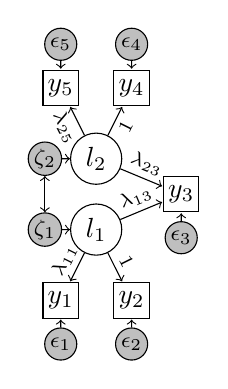
\begin{tikzpicture}[scale=0.9]	
	\begin{scope}	
		\node[latent] (ses) at (0,-0.5) {$l_1$};
		\node[latent] (stress) at (0,0.5) {$l_2$};
		\node[measure] (depression) at (1.2,0){$y_3$};
			
		%\draw[edge, <->] (ses) -- (stress) node[midway,above ] {\footnotesize $\beta_{12}$};
		\draw[edge] (ses) -- (depression) node[midway, above, sloped, yshift=-0.04cm] {\scriptsize $\lambda_{13}$};
		\draw[edge] (stress) -- (depression) node[midway, above, sloped, yshift=-0.04cm] {\scriptsize $\lambda_{23}$};
		
		% errors
		\node[error, inner sep=.5pt ] (zeta1) [left=.1cm of ses]  {\footnotesize $ \zeta_1 $};
		\node[error, inner sep=.5pt ] (zeta2) [left=.1cm of stress]  {\footnotesize $ \zeta_2 $};
		\node[error] (err3) [below=.1cm of depression]{\footnotesize $ \epsilon_3 $};
		\draw[edge] (err3) -- (depression);
		\draw[edge] (zeta1) -- (ses);
		\draw[edge] (zeta2) -- (stress);
		\draw[edge, <->] (zeta1) -- (zeta2);
			
		% Measurements of ses
		\begin{scope}[xshift=0cm, yshift=-1.5cm]	
			\node[measure] (edu) at (0.5,0) {$y_2$};
			\node[measure] (inc) at (-0.5,0) {$y_1$};
			\draw[edge] (ses) -- (edu) node[midway, above, sloped, yshift=-0.04cm ]{\scriptsize $1$ };
			\draw[edge] (ses) -- (inc) node[midway, above, sloped, yshift=-0.04cm ]{\scriptsize $\lambda_{11}$ };
			
			%errors
			\node[error] (err2) [below=.1cm of edu] {\footnotesize $ \epsilon_2 $};
			\node[error] (err1) [below=.1cm of inc] {\footnotesize $ \epsilon_1 $};
			\draw[edge] (err2) -- (edu);
			\draw[edge] (err1) -- (inc);
			
			%crossloading on income and education
			% \draw[edge, <->] (err2) -- (err1);	
		\end{scope}
		
		% Measurements of stress
		\begin{scope}[xshift=0cm, yshift=1.5cm]
			\node[measure] (ip) at (0.5,0) {$y_4$};
			\node[measure] (job) at (-0.5,0) {$y_5$};
			\draw[edge] (stress) -- (ip) node[midway, below, sloped, yshift=0.05cm ]{\scriptsize $1$ };
			\draw[edge] (stress) -- (job) node[midway, below, sloped, yshift=0.05cm ]{\scriptsize $\lambda_{25}$ };
			
			%errors
			\node[error] (err4) [above=.1cm of ip] {\footnotesize $ \epsilon_4 $};
			\node[error] (err5) [above=.1cm of job] {\footnotesize $ \epsilon_5 $};
			\draw[edge] (err4) -- (ip);
			\draw[edge] (err5) -- (job);
		\end{scope}	
	\end{scope}

\end{tikzpicture}

% Page 8: Transformed model for the LVSEM example.
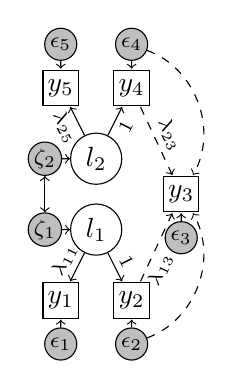
\begin{tikzpicture}[scale=0.9]
	
	\begin{scope}

		\node[latent] (ses) at (0,-0.5) {$l_1$};
		\node[latent] (stress) at (0,0.5) {$l_2$};
		\node[measure] (depression) at (1.2,0){$y_3$};
			
		%\draw[edge, <->] (ses) -- (stress) node[midway,above ] {\footnotesize $\beta_{12}$};
		% \draw[edge] (ses) -- (depression) node[midway, above, sloped, yshift=-0.04cm] {\scriptsize $\lambda_{13}$};
		% \draw[edge] (stress) -- (depression) node[near end, above] {\footnotesize $\lambda_{23}$};
		
		% errors
		\node[error, inner sep=.5pt ] (zeta1) [left=.1cm of ses]  {\footnotesize $ \zeta_1 $};
		\node[error, inner sep=.5pt ] (zeta2) [left=.1cm of stress]  {\footnotesize $ \zeta_2 $};
		\node[error] (err3) [below=.1cm of depression]{\footnotesize $ \epsilon_3 $};
		\draw[edge] (err3) -- (depression);
		\draw[edge] (zeta1) -- (ses);
		\draw[edge] (zeta2) -- (stress);
		\draw[edge, <->] (zeta1) -- (zeta2);

		% Measurements of ses
		\begin{scope}[xshift=0cm, yshift=-1.5cm]	
			\node[measure] (edu) at (0.5,0) {$y_2$};
			\node[measure] (inc) at (-0.5,0) {$y_1$};
			\draw[edge] (ses) -- (edu) node[midway, above, sloped, yshift=-0.04cm ] {\scriptsize $1$ };
			\draw[edge] (ses) -- (inc) node[midway, above, sloped, yshift=-0.04cm ] {\scriptsize $\lambda_{11}$ };
			
			%errors
			\node[error] (err2) [below=.1cm of edu] {\footnotesize $ \epsilon_2 $};
			\node[error] (err1) [below=.1cm of inc] {\footnotesize $ \epsilon_1 $};
			\draw[edge] (err2) -- (edu);
			\draw[edge] (err1) -- (inc);
			
			%crossloading on income and education
			%\draw[edge, <->] (err2) -- (err1);	
		\end{scope}
		
		% Measurements of stress
		\begin{scope}[xshift=0cm, yshift=1.5cm]
			\node[measure] (ip) at (0.5,0) {$y_4$};
			\node[measure] (job) at (-0.5,0) {$y_5$};
			\draw[edge] (stress) -- (ip) node[midway, below, sloped, yshift=0.05cm ]{\scriptsize $1$ };
			\draw[edge] (stress) -- (job) node[midway, below, sloped, yshift=0.05cm ]{\scriptsize $\lambda_{25}$ };
			
			%errors
			\node[error] (err4) [above=.1cm of ip] {\footnotesize $ \epsilon_4 $};
			\node[error] (err5) [above=.1cm of job] {\footnotesize $ \epsilon_5 $};
			\draw[edge] (err4) -- (ip);
			\draw[edge] (err5) -- (job);
		\end{scope}	

		%\node at (0,-1.8) {(a)};
		% Transformation edges
		\begin{scope}
			\draw[highlightEdge2] (ip) -- (depression) node[midway, above, sloped, yshift=-0.04cm]{\scriptsize $ \lambda_{23}$ };
			% \draw[highlightEdge2] (err2) edge [bend right=50] (depression);
			% \draw[highlightEdge2] (edu) -- (depression) node[midway, below,
			% sloped]{\footnotesize $ \lambda_{13} $ };
			\draw[highlightEdge2] (err4) edge [bend left=50] (depression);

			\draw[highlightEdge2] (edu) -- (depression) node[near start, below, sloped, yshift=0.06cm]{\scriptsize $\lambda_{13}$ };
			\draw[highlightEdge2] (err2) edge [bend right=50] (depression);
		\end{scope}
	
	\end{scope}

\end{tikzpicture}

% Page 9: Transformed model for the LVSEM example.
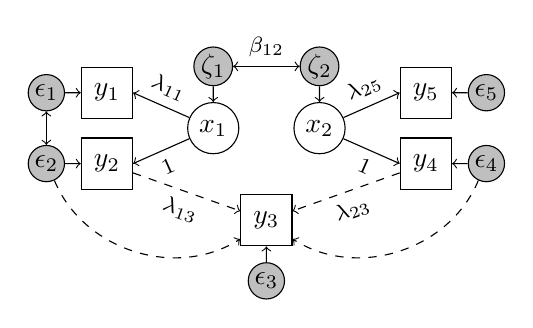
\begin{tikzpicture}[scale=0.9]
	
	\begin{scope}
	
		%\fill[ fill=gray!30!white, anchor = north west ] (-0.3,1.5) rectangle +(3.6,-2.35);
	
		%\node[anchor=north west] at (-0.3,1.5) {\itshape \small latent level};
		%\node[anchor=north east] at (-0.3,1.5) {\itshape \small observed level};

		\node[latent] (ses) at (0.5,0) {$x_1$};
		\node[latent] (stress) at (2,0) {$x_2$};
		\node[observed] (depression) at (1.25,-1.3){$y_3$};
		
		
		% \draw[edge, <->] (ses) -- (stress) node[midway,above ] {\footnotesize $\beta_{12}$};
		% \draw[edge] (ses) -- (depression) node[near end,left] {\footnotesize $\lambda_{13}$};
		% \draw[edge] (stress) -- (depression) node[near end, right] {\footnotesize $\lambda_{23}$};
		
		% errors
		\node[error, inner sep=.5pt ] (zeta1) [above=.2cm of ses]  {$ \zeta_1 $};
		\node[error, inner sep=.5pt ] (zeta2) [above=.2cm of stress]  {$ \zeta_2 $};
		\node[error] (err3) [below=.2cm of depression]{$ \epsilon_3 $};
		\draw[edge] (err3) -- (depression);
		\draw[edge] (zeta1) -- (ses);
		\draw[edge] (zeta2) -- (stress);
		\draw[edge, <->] (zeta1) -- (zeta2) node[midway,above]{\footnotesize $ \beta_{12} $};
		
		
		% Measurements of ses
		\begin{scope}[xshift=-1cm, yshift=0cm]
		
			\node[observed] (edu) at (0,-0.5) {$y_2$};
			\node[observed] (inc) at (0,0.5) {$y_1$};
			\draw[edge] (ses) -- (edu.east) node[midway, below, sloped ]
			{\footnotesize $1$ };
			\draw[edge] (ses) -- (inc.east) node[midway, above, sloped ]
			{\footnotesize $\lambda_{11}$ };
			
			%errors
			\node[error] (err2) [left=.2cm of edu] {$ \epsilon_2 $};
			\node[error] (err1) [left=.2cm of inc] {$ \epsilon_1 $};
			\draw[edge] (err2) -- (edu);
			\draw[edge] (err1) -- (inc);
			
			%crossloading on income and education
			\draw[edge, <->] (err2) -- (err1);
			
		\end{scope}
		
		% Measurements of stress
		\begin{scope}[xshift=3.5cm, yshift=0cm]
			\node[observed] (ip) at (0,-0.5) {$y_4$};
			\node[observed] (job) at (0,0.5) {$y_5$};
			\draw[edge] (stress) -- (ip.west) node[midway, below, sloped ]
			{\footnotesize $1$ };
			\draw[edge] (stress) -- (job.west) node[midway, above, sloped ]
			{\footnotesize $\lambda_{25}$ };
			
			%errors
			\node[error] (err4) [right=.2cm of ip] {$ \epsilon_4 $};
			\node[error] (err5) [right=.2cm of job] {$ \epsilon_5 $};
			\draw[edge] (err4) -- (ip);
			\draw[edge] (err5) -- (job);
		\end{scope}
		
		
		%\node at (0,-1.8) {(a)};
		% Transformation edges
		\begin{scope}
			\draw[highlightEdge2] (ip) -- (depression) node[midway, below,
			sloped]{\footnotesize $ \lambda_{23}$ };
			\draw[highlightEdge2] (err2) edge [bend right=50] (depression);
			\draw[highlightEdge2] (edu) -- (depression) node[midway, below,
			sloped]{\footnotesize $ \lambda_{13} $ };
			\draw[highlightEdge2] (err4) edge [bend left=50] (depression);
		\end{scope}
	
	\end{scope}

\end{tikzpicture}


% Page 10: Transformed model for the LVSEM example with $ x_1 $ as the only covariate.
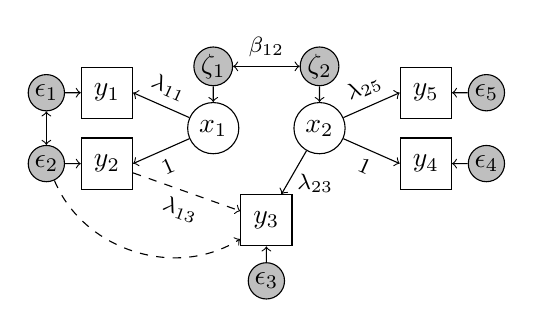
\begin{tikzpicture}[scale=0.9]
	
	\begin{scope}
	
		%\fill[ fill=gray!30!white, anchor = north west ] (-0.3,1.5) rectangle +(3.6,-2.35);
	
		%\node[anchor=north west] at (-0.3,1.5) {\itshape \small latent level};
		%\node[anchor=north east] at (-0.3,1.5) {\itshape \small observed level};

		\node[latent] (ses) at (0.5,0) {$x_1$};
		\node[latent] (stress) at (2,0) {$x_2$};
		\node[observed] (depression) at (1.25,-1.3){$y_3$};
		
		
		% \draw[edge, <->] (ses) -- (stress) node[midway,above ] {\footnotesize $\beta_{12}$};
		% \draw[edge] (ses) -- (depression) node[near end,left] {\footnotesize $\lambda_{13}$};
		\draw[edge] (stress) -- (depression) node[near end, right] {\footnotesize $\lambda_{23}$};
		
		% errors
		\node[error, inner sep=.5pt ] (zeta1) [above=.2cm of ses]  {$ \zeta_1 $};
		\node[error, inner sep=.5pt ] (zeta2) [above=.2cm of stress]  {$ \zeta_2 $};
		\node[error] (err3) [below=.2cm of depression]{$ \epsilon_3 $};
		\draw[edge] (err3) -- (depression);
		\draw[edge] (zeta1) -- (ses);
		\draw[edge] (zeta2) -- (stress);	
		\draw[edge, <->] (zeta1) -- (zeta2) node[midway,above]{\footnotesize $ \beta_{12} $};
		
		% Measurements of ses
		\begin{scope}[xshift=-1cm, yshift=0cm]
		
			\node[observed] (edu) at (0,-0.5) {$y_2$};
			\node[observed] (inc) at (0,0.5) {$y_1$};
			\draw[edge] (ses) -- (edu.east) node[midway, below, sloped ]
			{\footnotesize $1$ };
			\draw[edge] (ses) -- (inc.east) node[midway, above, sloped ]
			{\footnotesize $\lambda_{11}$ };
			
			%errors
			\node[error] (err2) [left=.2cm of edu] {$ \epsilon_2 $};
			\node[error] (err1) [left=.2cm of inc] {$ \epsilon_1 $};
			\draw[edge] (err2) -- (edu);
			\draw[edge] (err1) -- (inc);
			
			%crossloading on income and education
			\draw[edge, <->] (err2) -- (err1);
			
		\end{scope}
		
		% Measurements of stress
		\begin{scope}[xshift=3.5cm, yshift=0cm]
			\node[observed] (ip) at (0,-0.5) {$y_4$};
			\node[observed] (job) at (0,0.5) {$y_5$};
			\draw[edge] (stress) -- (ip.west) node[midway, below, sloped ]
			{\footnotesize $1$ };
			\draw[edge] (stress) -- (job.west) node[midway, above, sloped ]
			{\footnotesize $\lambda_{25}$ };
			
			%errors
			\node[error] (err4) [right=.2cm of ip] {$ \epsilon_4 $};
			\node[error] (err5) [right=.2cm of job] {$ \epsilon_5 $};
			\draw[edge] (err4) -- (ip);
			\draw[edge] (err5) -- (job);
		\end{scope}
		
		
		%\node at (0,-1.8) {(a)};
		% Transformation edges
		\begin{scope}
			% \draw[highlightEdge2] (ip) -- (depression) node[midway, below,
			% sloped]{\footnotesize $ \lambda_{23}$ };
			\draw[highlightEdge2] (err2) edge [bend right=50] (depression);
			\draw[highlightEdge2] (edu) -- (depression) node[midway, below,
			sloped]{\footnotesize $ \lambda_{13} $ };
			% \draw[highlightEdge2] (err4) edge [bend left=50] (depression);
		\end{scope}
	
	\end{scope}

\end{tikzpicture}

% Page 11: Example model for the example with non-correlated latents.
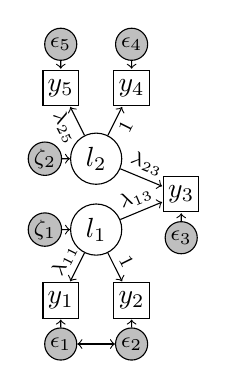
\begin{tikzpicture}[scale=0.9]	
	\begin{scope}	
		\node[latent] (ses) at (0,-0.5) {$l_1$};
		\node[latent] (stress) at (0,0.5) {$l_2$};
		\node[measure] (depression) at (1.2,0){$y_3$};
			
		%\draw[edge, <->] (ses) -- (stress) node[midway,above ] {\footnotesize $\beta_{12}$};
		\draw[edge] (ses) -- (depression) node[midway, above, sloped, yshift=-0.04cm] {\scriptsize $\lambda_{13}$};
		\draw[edge] (stress) -- (depression) node[midway, above, sloped, yshift=-0.04cm] {\scriptsize $\lambda_{23}$};
		
		% errors
		\node[error, inner sep=.5pt ] (zeta1) [left=.1cm of ses]  {\footnotesize $ \zeta_1 $};
		\node[error, inner sep=.5pt ] (zeta2) [left=.1cm of stress]  {\footnotesize $ \zeta_2 $};
		\node[error] (err3) [below=.1cm of depression]{\footnotesize $ \epsilon_3 $};
		\draw[edge] (err3) -- (depression);
		\draw[edge] (zeta1) -- (ses);
		\draw[edge] (zeta2) -- (stress);
			
		% Measurements of ses
		\begin{scope}[xshift=0cm, yshift=-1.5cm]	
			\node[measure] (edu) at (0.5,0) {$y_2$};
			\node[measure] (inc) at (-0.5,0) {$y_1$};
			\draw[edge] (ses) -- (edu) node[midway, above, sloped, yshift=-0.04cm ]{\scriptsize $1$ };
			\draw[edge] (ses) -- (inc) node[midway, above, sloped, yshift=-0.04cm ]{\scriptsize $\lambda_{11}$ };
			
			%errors
			\node[error] (err2) [below=.1cm of edu] {\footnotesize $ \epsilon_2 $};
			\node[error] (err1) [below=.1cm of inc] {\footnotesize $ \epsilon_1 $};
			\draw[edge] (err2) -- (edu);
			\draw[edge] (err1) -- (inc);
			
			%crossloading on income and education
			\draw[edge, <->] (err2) -- (err1);	
		\end{scope}
		
		% Measurements of stress
		\begin{scope}[xshift=0cm, yshift=1.5cm]
			\node[measure] (ip) at (0.5,0) {$y_4$};
			\node[measure] (job) at (-0.5,0) {$y_5$};
			\draw[edge] (stress) -- (ip) node[midway, below, sloped, yshift=0.05cm ]{\scriptsize $1$ };
			\draw[edge] (stress) -- (job) node[midway, below, sloped, yshift=0.05cm ]{\scriptsize $\lambda_{25}$ };
			
			%errors
			\node[error] (err4) [above=.1cm of ip] {\footnotesize $ \epsilon_4 $};
			\node[error] (err5) [above=.1cm of job] {\footnotesize $ \epsilon_5 $};
			\draw[edge] (err4) -- (ip);
			\draw[edge] (err5) -- (job);
		\end{scope}	
	\end{scope}

\end{tikzpicture}


% Page 12: Transformed model for the example with non-correlated latents.
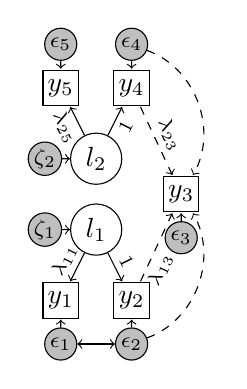
\begin{tikzpicture}[scale=0.9]
	
	\begin{scope}

		\node[latent] (ses) at (0,-0.5) {$l_1$};
		\node[latent] (stress) at (0,0.5) {$l_2$};
		\node[measure] (depression) at (1.2,0){$y_3$};
			
		%\draw[edge, <->] (ses) -- (stress) node[midway,above ] {\footnotesize $\beta_{12}$};
		% \draw[edge] (ses) -- (depression) node[midway, above, sloped, yshift=-0.04cm] {\scriptsize $\lambda_{13}$};
		% \draw[edge] (stress) -- (depression) node[near end, above] {\footnotesize $\lambda_{23}$};
		
		% errors
		\node[error, inner sep=.5pt ] (zeta1) [left=.1cm of ses]  {\footnotesize $ \zeta_1 $};
		\node[error, inner sep=.5pt ] (zeta2) [left=.1cm of stress]  {\footnotesize $ \zeta_2 $};
		\node[error] (err3) [below=.1cm of depression]{\footnotesize $ \epsilon_3 $};
		\draw[edge] (err3) -- (depression);
		\draw[edge] (zeta1) -- (ses);
		\draw[edge] (zeta2) -- (stress);

		% Measurements of ses
		\begin{scope}[xshift=0cm, yshift=-1.5cm]	
			\node[measure] (edu) at (0.5,0) {$y_2$};
			\node[measure] (inc) at (-0.5,0) {$y_1$};
			\draw[edge] (ses) -- (edu) node[midway, above, sloped, yshift=-0.04cm ] {\scriptsize $1$ };
			\draw[edge] (ses) -- (inc) node[midway, above, sloped, yshift=-0.04cm ] {\scriptsize $\lambda_{11}$ };
			
			%errors
			\node[error] (err2) [below=.1cm of edu] {\footnotesize $ \epsilon_2 $};
			\node[error] (err1) [below=.1cm of inc] {\footnotesize $ \epsilon_1 $};
			\draw[edge] (err2) -- (edu);
			\draw[edge] (err1) -- (inc);
			
			%crossloading on income and education
			\draw[edge, <->] (err2) -- (err1);	
		\end{scope}
		
		% Measurements of stress
		\begin{scope}[xshift=0cm, yshift=1.5cm]
			\node[measure] (ip) at (0.5,0) {$y_4$};
			\node[measure] (job) at (-0.5,0) {$y_5$};
			\draw[edge] (stress) -- (ip) node[midway, below, sloped, yshift=0.05cm ]{\scriptsize $1$ };
			\draw[edge] (stress) -- (job) node[midway, below, sloped, yshift=0.05cm ]{\scriptsize $\lambda_{25}$ };
			
			%errors
			\node[error] (err4) [above=.1cm of ip] {\footnotesize $ \epsilon_4 $};
			\node[error] (err5) [above=.1cm of job] {\footnotesize $ \epsilon_5 $};
			\draw[edge] (err4) -- (ip);
			\draw[edge] (err5) -- (job);
		\end{scope}	

		%\node at (0,-1.8) {(a)};
		% Transformation edges
		\begin{scope}
			\draw[highlightEdge2] (ip) -- (depression) node[midway, above, sloped, yshift=-0.04cm]{\scriptsize $ \lambda_{23}$ };
			% \draw[highlightEdge2] (err2) edge [bend right=50] (depression);
			% \draw[highlightEdge2] (edu) -- (depression) node[midway, below,
			% sloped]{\footnotesize $ \lambda_{13} $ };
			\draw[highlightEdge2] (err4) edge [bend left=50] (depression);

			\draw[highlightEdge2] (edu) -- (depression) node[near start, below, sloped, yshift=0.06cm]{\scriptsize $\lambda_{13}$ };
			\draw[highlightEdge2] (err2) edge [bend right=50] (depression);
		\end{scope}
	
	\end{scope}

\end{tikzpicture}

% Page 13: Transformed model for the example with non-correlated latents.
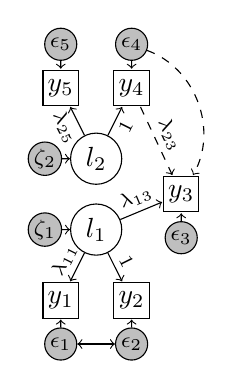
\begin{tikzpicture}[scale=0.9]
	
	\begin{scope}

		\node[latent] (ses) at (0,-0.5) {$l_1$};
		\node[latent] (stress) at (0,0.5) {$l_2$};
		\node[measure] (depression) at (1.2,0){$y_3$};
			
		%\draw[edge, <->] (ses) -- (stress) node[midway,above ] {\footnotesize $\beta_{12}$};
		\draw[edge] (ses) -- (depression) node[midway, above, sloped, yshift=-0.04cm] {\scriptsize $\lambda_{13}$};
		% \draw[edge] (stress) -- (depression) node[near end, above] {\footnotesize $\lambda_{23}$};
		
		% errors
		\node[error, inner sep=.5pt ] (zeta1) [left=.1cm of ses]  {\footnotesize $ \zeta_1 $};
		\node[error, inner sep=.5pt ] (zeta2) [left=.1cm of stress]  {\footnotesize $ \zeta_2 $};
		\node[error] (err3) [below=.1cm of depression]{\footnotesize $ \epsilon_3 $};
		\draw[edge] (err3) -- (depression);
		\draw[edge] (zeta1) -- (ses);
		\draw[edge] (zeta2) -- (stress);

		% Measurements of ses
		\begin{scope}[xshift=0cm, yshift=-1.5cm]	
			\node[measure] (edu) at (0.5,0) {$y_2$};
			\node[measure] (inc) at (-0.5,0) {$y_1$};
			\draw[edge] (ses) -- (edu) node[midway, above, sloped, yshift=-0.04cm ] {\scriptsize $1$ };
			\draw[edge] (ses) -- (inc) node[midway, above, sloped, yshift=-0.04cm ] {\scriptsize $\lambda_{11}$ };
			
			%errors
			\node[error] (err2) [below=.1cm of edu] {\footnotesize $ \epsilon_2 $};
			\node[error] (err1) [below=.1cm of inc] {\footnotesize $ \epsilon_1 $};
			\draw[edge] (err2) -- (edu);
			\draw[edge] (err1) -- (inc);
			
			%crossloading on income and education
			\draw[edge, <->] (err2) -- (err1);	
		\end{scope}
		
		% Measurements of stress
		\begin{scope}[xshift=0cm, yshift=1.5cm]
			\node[measure] (ip) at (0.5,0) {$y_4$};
			\node[measure] (job) at (-0.5,0) {$y_5$};
			\draw[edge] (stress) -- (ip) node[midway, below, sloped, yshift=0.05cm ]{\scriptsize $1$ };
			\draw[edge] (stress) -- (job) node[midway, below, sloped, yshift=0.05cm ]{\scriptsize $\lambda_{25}$ };
			
			%errors
			\node[error] (err4) [above=.1cm of ip] {\footnotesize $ \epsilon_4 $};
			\node[error] (err5) [above=.1cm of job] {\footnotesize $ \epsilon_5 $};
			\draw[edge] (err4) -- (ip);
			\draw[edge] (err5) -- (job);
		\end{scope}	

		%\node at (0,-1.8) {(a)};
		% Transformation edges
		\begin{scope}
			\draw[highlightEdge2] (ip) -- (depression) node[midway, above, sloped, yshift=-0.04cm]{\scriptsize $ \lambda_{23}$ };
			% \draw[highlightEdge2] (err2) edge [bend right=50] (depression);
			% \draw[highlightEdge2] (edu) -- (depression) node[midway, below,
			% sloped]{\footnotesize $ \lambda_{13} $ };
			\draw[highlightEdge2] (err4) edge [bend left=50] (depression);
		\end{scope}
	
	\end{scope}

\end{tikzpicture}

% Page 14: Example model for conditional IV.
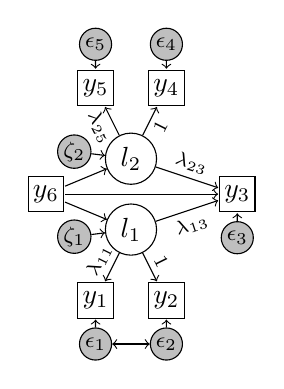
\begin{tikzpicture}[scale=0.9]
	
	\begin{scope}
	
		%\fill[ fill=gray!30!white, anchor = north west ] (-0.3,1.5) rectangle +(3.6,-2.35);
	
		%\node[anchor=north west] at (-0.3,1.5) {\itshape \small latent level};
		%\node[anchor=north east] at (-0.3,1.5) {\itshape \small observed level};

		\node[latent] (ses) at (0,-0.5) {$l_1$};
		\node[latent] (stress) at (0,0.5) {$l_2$};
		\node[measure] (depression) at (1.5,0){$y_3$};
		\node[measure] (condition) at (-1.2, 0){$y_6$};
		
		
		%\draw[edge, <->] (ses) -- (stress) node[midway,above ] {\footnotesize $\beta_{12}$};
		\draw[edge] (condition) -- (ses);
		\draw[edge] (condition) -- (stress);
		\draw[edge] (ses) -- (depression) node[midway, below, sloped, yshift=0.04cm] {\scriptsize $\lambda_{13}$};
		\draw[edge] (stress) -- (depression) node[midway, above, sloped, yshift=-0.04cm] {\scriptsize $\lambda_{23}$};
		\draw[edge] (condition) -- (depression);
		
		% errors
		\node[error, inner sep=.5pt ] (zeta1) at (-0.8, -0.6) {\footnotesize $ \zeta_1 $};
		\node[error, inner sep=.5pt ] (zeta2) at (-0.8, 0.6) {\footnotesize $ \zeta_2 $};
		\node[error] (err3) [below=.1cm of depression]{\footnotesize $ \epsilon_3 $};
		\draw[edge] (err3) -- (depression);
		\draw[edge] (zeta1) -- (ses);
		\draw[edge] (zeta2) -- (stress);
		
		
		% Measurements of ses
		\begin{scope}[xshift=0cm, yshift=-1.5cm]
		
			\node[measure] (edu) at (0.5,0) {$y_2$};
			\node[measure] (inc) at (-0.5,0) {$y_1$};
			\draw[edge] (ses) -- (edu) node[midway, above, sloped, yshift=-0.04cm]{\scriptsize $1$ };
			\draw[edge] (ses) -- (inc) node[midway, above, sloped, yshift=-0.04cm]{\scriptsize $\lambda_{11}$ };
			
			%errors
			\node[error] (err2) [below=.1cm of edu] {\footnotesize $ \epsilon_2 $};
			\node[error] (err1) [below=.1cm of inc] {\footnotesize $ \epsilon_1 $};
			\draw[edge] (err2) -- (edu);
			\draw[edge] (err1) -- (inc);
			
			%crossloading on income and education
			\draw[edge, <->] (err2) -- (err1);
			
		\end{scope}
		
		% Measurements of stress
		\begin{scope}[xshift=0cm, yshift=1.5cm]
			\node[measure] (ip) at (0.5,0) {$y_4$};
			\node[measure] (job) at (-0.5,0) {$y_5$};
			\draw[edge] (stress) -- (ip) node[midway, below, sloped, yshift=0.05cm]{\scriptsize $1$ };
			\draw[edge] (stress) -- (job) node[midway, below, sloped, yshift=0.05cm]{\scriptsize $\lambda_{25}$ };
			
			%errors
			\node[error] (err4) [above=.1cm of ip] {\footnotesize $ \epsilon_4 $};
			\node[error] (err5) [above=.1cm of job] {\footnotesize $ \epsilon_5 $};
			\draw[edge] (err4) -- (ip);
			\draw[edge] (err5) -- (job);
		\end{scope}	
	\end{scope}

\end{tikzpicture}

% Page 14: Transformed model for the example with conditional IV.
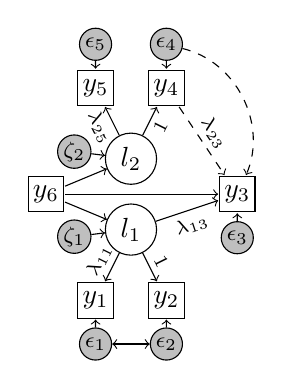
\begin{tikzpicture}[scale=0.9]
	
	\begin{scope}
		\node[latent] (ses) at (0,-0.5) {$l_1$};
		\node[latent] (stress) at (0,0.5) {$l_2$};
		\node[measure] (depression) at (1.5,0){$y_3$};
		\node[measure] (condition) at (-1.2, 0){$y_6$};
			
		\draw[edge] (condition) -- (ses);
		\draw[edge] (condition) -- (stress);
		\draw[edge] (ses) -- (depression) node[midway,below, sloped, yshift=0.04cm] {\scriptsize $\lambda_{13}$};
		\draw[edge] (condition) -- (depression);
		
		% errors
		\node[error, inner sep=.5pt ] (zeta1) at (-0.8, -0.6) {\footnotesize $ \zeta_1 $};
		\node[error, inner sep=.5pt ] (zeta2) at (-0.8, 0.6) {\footnotesize $ \zeta_2 $};
		\node[error] (err3) [below=.1cm of depression]{\footnotesize $ \epsilon_3 $};
		\draw[edge] (err3) -- (depression);
		\draw[edge] (zeta1) -- (ses);
		\draw[edge] (zeta2) -- (stress);
		
		
		% Measurements of ses
		\begin{scope}[xshift=0cm, yshift=-1.5cm]
		
			\node[measure] (edu) at (0.5,0) {$y_2$};
			\node[measure] (inc) at (-0.5,0) {$y_1$};
			\draw[edge] (ses) -- (edu) node[midway, above, sloped, yshift=-0.04cm] {\scriptsize $1$ };
			\draw[edge] (ses) -- (inc) node[midway, above, sloped, yshift=-0.04cm] {\scriptsize $\lambda_{11}$ };
			
			%errors
			\node[error] (err2) [below=.1cm of edu] {\footnotesize $ \epsilon_2 $};
			\node[error] (err1) [below=.1cm of inc] {\footnotesize $ \epsilon_1 $};
			\draw[edge] (err2) -- (edu);
			\draw[edge] (err1) -- (inc);
			
			%crossloading on income and education
			\draw[edge, <->] (err2) -- (err1);
			
		\end{scope}
		
		% Measurements of stress
		\begin{scope}[xshift=0cm, yshift=1.5cm]
			\node[measure] (ip) at (0.5,0) {$y_4$};
			\node[measure] (job) at (-0.5,0) {$y_5$};
			\draw[edge] (stress) -- (ip) node[midway, below, sloped, yshift=0.05cm]{\scriptsize $1$ };
			\draw[edge] (stress) -- (job) node[midway, below, sloped, yshift=0.05cm]{\scriptsize $\lambda_{25}$ };
			
			%errors
			\node[error] (err4) [above=.1cm of ip] {\footnotesize $ \epsilon_4 $};
			\node[error] (err5) [above=.1cm of job] {\footnotesize $ \epsilon_5 $};
			\draw[edge] (err4) -- (ip);
			\draw[edge] (err5) -- (job);
		\end{scope}	

		% Transformation edges
		\begin{scope}
			\draw[highlightEdge2] (ip) -- (depression) node[midway, above, sloped, yshift=-0.04cm]{\scriptsize $ \lambda_{23}$ };
			\draw[highlightEdge2] (err4) edge [bend left=50] (depression);
		\end{scope}
	
	\end{scope}

\end{tikzpicture}


%%%%% Example where the parameter gets changed.
% Example of the original model
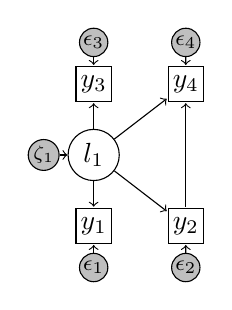
\begin{tikzpicture}[scale=0.9]
	% variable nodes
	\node[latent] (ability) at (0,0) {$l_1$};
	\node[measure] (iq) at (0, -1) {$y_1$};
	\node[measure] (schooling) at (1.3,-1){$y_2$};
	\node[measure] (kww) at (0, 1){$y_3$};
	\node[measure] (income) at (1.3, 1){$y_4$};

	% Error nodes
	\node[error, inner sep=.5pt ] (zeta1) [left=.1cm of ability]  {\scriptsize $ \zeta_1 $};
	\node[error, inner sep=.5pt ] (epsilon1) [below=.1cm of iq]  {\footnotesize $ \epsilon_1$};
	\node[error, inner sep=.5pt ] (epsilon2) [below=.1cm of schooling]  {\footnotesize $ \epsilon_2$};
	\node[error, inner sep=.5pt ] (epsilon3) [above=.1cm of kww]  {\footnotesize $ \epsilon_3$};
	\node[error, inner sep=.5pt ] (epsilon4) [above=.1cm of income]  {\footnotesize $ \epsilon_4$};

	% variable edges
	\draw[edge] (ability) -- (iq); 
	\draw[edge] (ability) -- (kww);
	\draw[edge] (ability) -- (schooling);
	\draw[edge] (ability) -- (income);
	\draw[edge] (schooling) -- (income);


	% Error edges
	\draw[edge] (zeta1) -- (ability);
	\draw[edge] (epsilon1) -- (iq);
	\draw[edge] (epsilon2) -- (schooling);
	\draw[edge] (epsilon3) -- (kww);
	\draw[edge] (epsilon4) -- (income);

\end{tikzpicture}

% Example of incorrect parameter estimation
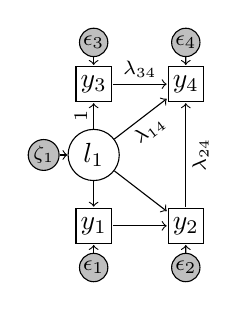
\begin{tikzpicture}[scale=0.9]
	% variable nodes
	\node[latent] (ability) at (0,0) {$l_1$};
	\node[measure] (iq) at (0, -1) {$y_1$};
	\node[measure] (schooling) at (1.3,-1){$y_2$};
	\node[measure] (kww) at (0, 1){$y_3$};
	\node[measure] (income) at (1.3, 1){$y_4$};

	% Error nodes
	\node[error, inner sep=.5pt ] (zeta1) [left=.1cm of ability]  {\scriptsize $ \zeta_1 $};
	\node[error, inner sep=.5pt ] (epsilon1) [below=.1cm of iq]  {\footnotesize $ \epsilon_1$};
	\node[error, inner sep=.5pt ] (epsilon2) [below=.1cm of schooling]  {\footnotesize $ \epsilon_2$};
	\node[error, inner sep=.5pt ] (epsilon3) [above=.1cm of kww]  {\footnotesize $ \epsilon_3$};
	\node[error, inner sep=.5pt ] (epsilon4) [above=.1cm of income]  {\footnotesize $ \epsilon_4$};
	
	% variable edges
	\draw[edge] (ability) -- (iq); 
	\draw[edge] (ability) -- (kww) node[midway, above, sloped, yshift=-0.04cm] {\scriptsize $1$};
	\draw[edge] (ability) -- (schooling);
	\draw[edge] (iq) -- (schooling);
	\draw[edge] (ability) -- (income) node[midway, below, sloped, yshift=0.04cm] 
        			{\scriptsize $\lambda_{14}$};
	\draw[edge] (kww) -- (income) node[midway, above, sloped, yshift=-0.04cm]
				{\scriptsize $\lambda_{34}$};
	\draw[edge] (schooling) -- (income) node[midway, below, sloped, yshift=0.04cm]
				{\scriptsize $\lambda_{24}$};

	% Error edges
	\draw[edge] (zeta1) -- (ability);
	\draw[edge] (epsilon1) -- (iq);
	\draw[edge] (epsilon2) -- (schooling);
	\draw[edge] (epsilon3) -- (kww);
	\draw[edge] (epsilon4) -- (income);

\end{tikzpicture}

% Transformed example of incorrect parameter estimation
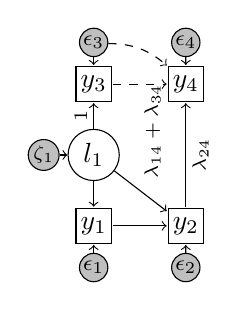
\begin{tikzpicture}[scale=0.9]
	% variable nodes
	\node[latent] (ability) at (0,0) {$l_1$};
	\node[measure] (iq) at (0, -1) {$y_1$};
	\node[measure] (schooling) at (1.3,-1){$y_2$};
	\node[measure] (kww) at (0, 1){$y_3$};
	\node[measure] (income) at (1.3, 1){$y_4$};

	% Error nodes
	\node[error, inner sep=.5pt ] (zeta1) [left=.1cm of ability]  {\scriptsize $ \zeta_1 $};
	\node[error, inner sep=.5pt ] (epsilon1) [below=.1cm of iq]  {\footnotesize $ \epsilon_1$};
	\node[error, inner sep=.5pt ] (epsilon2) [below=.1cm of schooling]  {\footnotesize $ \epsilon_2$};
	\node[error, inner sep=.5pt ] (epsilon3) [above=.1cm of kww]  {\footnotesize $ \epsilon_3$};
	\node[error, inner sep=.5pt ] (epsilon4) [above=.1cm of income]  {\footnotesize $ \epsilon_4$};

	% variable edges
	\draw[edge] (ability) -- (iq);
	\draw[edge] (ability) -- (kww) node[midway, above, sloped, yshift=-0.04cm] {\scriptsize $ 1 $ };
	\draw[edge] (ability) -- (schooling);
	\draw[edge] (iq) -- (schooling);
	\draw[highlightEdge2] (kww) -- (income) node[near end, rotate=90, xshift=-0.6cm, yshift=0.01cm]
				{\scriptsize $\lambda_{14} + \lambda_{34}$};
	\draw[edge] (schooling) -- (income) node[midway, below, sloped, yshift=0.04cm]
				{\scriptsize $\lambda_{24}$};

	% Error edges
	\draw[edge] (zeta1) -- (ability);
	\draw[edge] (epsilon1) -- (iq);
	\draw[edge] (epsilon2) -- (schooling);
	\draw[edge] (epsilon3) -- (kww);
	\draw[highlightEdge2] (epsilon3) edge [bend left = 20] (income);
	\draw[edge] (epsilon4) -- (income);

\end{tikzpicture}

\end{document}

